\chapter{REFERENCIAL TEÓRICO}
\label{cap:fundamentacao-teorica}


   A fundamentação teórica necessária para o entendimento e o embasamento deste trabalho é apresentada nas seções seguintes.

\begin{comment}
\subsection{Engenharia de software}

    A engenharia de software é uma área de estudo que surgiu devido a necessidade de profissionalizar a construção de sistemas computacionais. Esta necessidade é consequência da crescente adesão a alternativas tecnológicas e automatização de serviços pela sociedade atual. Portanto, a existência de uma metodologia de construção de sistemas mostrou-se cada vez mais necessária.
    
    Esta área abrange atividades, práticas e processos para o desenvolvimento de software e aplicativos. Ela define conceitos básicos a serem seguidos na construção de um software como: requisitos, arquitetura, implementação, teste e manutenção \cite{sommerville}.
    %, gerenciamento de projetos, testes em sistemas, arquitetura, manutenção de sistemas, dentre outros aspectos \cite{sommerville}.
   
    Os requisitos são dados coletados do cliente, que dizem respeito as exigências do mesmo. Eles correspondem a forma de como o cliente quer seu produto, a fase de arquitetura envolve a análise dos riscos, dos componentes e tecnologias a serem utilizadas, dentre outros aspectos. 
    
    Na implementação, é realizada a codificação do sistema baseado na arquitetura definida com o objetivo de atender aos requisitos levantados. Nos testes, é conduzida uma verificação se há erros no código podendo haver também uma validação de coerência com os requisitos. Finalmente, a manutenção compreende a busca de melhoria e otimização do produto final como também correções de erros. 
    
    Um sistema que é construído de acordo com as boas práticas da engenharia de software tem maior probabilidade de atender as necessidades do cliente e de ser mais aperfeiçoado do que os sistemas que não passam pelas etapas propostas por esta área.
    
    Todos esses procedimentos, estudos, a utilização de ferramentas, processos e metodologias ilustrados na Figura \ref{fig:camadas} tem como objetivo atingir um nível considerável de qualidade de software. Sendo assim, pode-se afirmar que a engenharia de software está altamente ligada ao desenvolvimento de software com alta qualidade.
   
     
    
\begin{figure}[h!] %use h para forçar que a figura fique abaixo do texto
	\caption{Camadas da engenharia de software.}
	\begin{center}
	    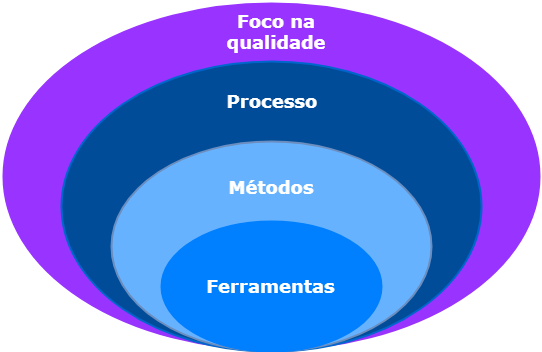
\includegraphics[scale=0.4]{figuras/camadas.png} % altere o atributo scale para o tamanho da figura
	\end{center}
	\label{fig:camadas}
	\legend{Fonte: Adaptado de \cite{pressman2005software}}
    \end{figure}
    
   Portanto, como a estrutura da sociedade hoje é dependente de sistemas computacionais, a engenharia de software é essencial nesse contexto. Esta área é responsável por cumprir estudos sobre como conhecer formas de construir, arquitetar e manter tais sistemas, tornando essencial no mundo moderno. Este trabalho é um estudo que está inserido na engenharia de software e se utilizará de conceitos da engenharia de requisitos. 
\end{comment}

     
\section{Engenharia de requisitos}

Visto que um software bem produzido é aquele que atende as necessidades do cliente, é necessário construir o sistema tendo um embasamento em fatos e informações reais. Sendo assim, a engenharia de requisitos é uma área da engenharia de software que pretende atingir esses objetivos. Esta área trata-se de um campo de estudo na engenharia de software de grande valia para o desenvolvimento de software.

    A engenharia de requisitos inclui atividades e etapas com o intuito de garantir que os requisitos reflitam as reais necessidades do solicitante. De acordo com \cite{kotonya}, o processo de engenharia de requisitos é composto por cinco etapas que são apresentadas na Figura \ref{fig:etapasRE}. 
    
    
    \begin{figure}[h!] %use h para forçar que a figura fique abaixo do texto
	\caption{Etapas da engenharia de requisitos.}
	\begin{center}
	    
\includegraphics[scale=0.8]{figuras/ER} % altere o atributo scale para o tamanho da figura
	\end{center}
	\label{fig:etapasRE}
	\legend{Fonte: Adaptado de \cite{kotonya}.}
\end{figure}
    
    A elicitação consiste em identificar e coletar as informações e o escopo do projeto que serão refinados e classificados na etapa de análise e negociação. Na especificação, é realizado uma descrição das funcionalidades e restrições do sistema a partir do resultado da fase de análise. Na etapa de validação, os requisitos serão verificados se estão de acordo com as necessidades dos \emph{stakeholders}. Finalmente, a fase de gerenciamento aborda questões relacionadas a evolução e rastreamento dos requisitos.
    
    Por ser um processo dinâmico e eficiente, a engenharia de requisitos é adotada amplamente no desenvolvimento de software, suprindo desde o estudo de viabilidade até a elaboração do documento de requisitos. As práticas adotadas nesta fase do processo de desenvolvimento de software são indispensáveis e de benefícios imensuráveis para projetos e empresas.
    
    A definição de requisitos requer a comunicação e colaboração de diversos \emph{stakeholders}. O processo de comunicação é descrito na próxima seção.
\section{Teoria da comunicação} \label{sec:fund_comunicacao}

A teoria da comunicação é uma área de pesquisa bastante abrangente que diz respeito aos efeitos da comunicação em todo o meio tecnológico, social, entre outros. Esta teoria define dois aspectos distintos \cite{pernstal}: um referindo-se ao processo da comunicação em si sendo retratado na troca de mensagens entre duas partes; e o outro ao significado do conteúdo ou ideia que está sendo transmitida.

No primeiro caso, a comunicação é analisada como um processo de transferência de informações entre os indivíduos ou partes (por exemplo, pessoas, grupos, organizações, documentos, etc.). Apesar de existir vários processos para descrever a comunicação, existem os seguintes pontos em comum \cite{pernstal}:

\begin{itemize}
    \item Remetente - quem está enviando a mensagem? 
    \item Mensagem - o que está sendo comunicado?
    \item Receptor - quem é o destinatário da mensagem?
    \item Canal de comunicação - como a mensagem é transmitida?
    \item Efeito - o resultado final da comunicação.
\end{itemize}

Também é importante ressaltar os seguintes conceitos:

\begin{itemize}
    \item Codificação – é a forma como o pensamento é processado. É transformar a informação em algo conhecido que será transferido.
    \item Decodificação – processo pelo qual o receptor ``traduz'' a informação emitida pelo emissor. Essa tradução vai depender de diversos fatores sendo de crucial importância no processo.
\end{itemize}

Esses conceitos envolvidos na comunicação são ilustrados na Figura \ref{fig:processocomunicacao}. Um elementos adicional nesse processo de comunicação pode ser uma fonte de ruído que é o termo utilizado quando algo é capaz de mudar ou distorcer a mensagem original do remetente \cite{pernstal}. 

\begin{figure}[h!] 
   	    \captionsetup{width=13cm}%Da mesma largura que a figura
		\Caption{\label{fig:processocomunicacao} Exemplo processo de comunicação.}
		\UFCfig{}{
			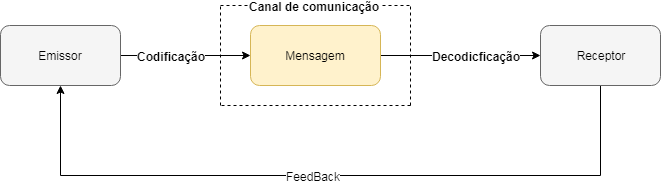
\includegraphics[width=13cm]{figuras/processoComunicacao.png}
		}{
			\Fonte{Fonte: Elaborado pelo autor }
		}	
	\end{figure}




A comunicação inserida no contexto de desenvolvimento de software é crucial para um projeto bem-sucedido \cite{pernstal, liskin2015artifacts}. A combinação da comunicação formal (por exemplo, documentos escritos e reuniões planejadas) e comunicação informal (por exemplo, reuniões presenciais não planejadas e outros meios convencionais como e-mails e redes sociais) interna e externamente em equipes, trata-se de um aspecto bastante vantajoso. 


\section{Comunicação de requisitos}

    A comunicação de requisitos se refere à capacidade das informações serem repassadas no processo de engenharia de requisitos, entre diferentes \emph{stakeholders}. Portanto, pode ser definida como a forma como o processo de comunicação atua na engenharia de requisitos. É de fundamental importância agilizar o processo. Quando a comunicação é falha, o projeto estará sujeito a atrasos, erros, ineficiência entre outros fatores.
    
Os canais de comunicação de requisitos são bastante variados podendo ser, por exemplo: 
    
\begin{itemize}
    \item Artefatos (documentos, modelos) gerados no processo;
    \item Ferramentas de comunicação;
    \item Reuniões (planejadas e não planejadas);
    \item Conversas informais e formais.
\end{itemize}

    Durante a comunicação, é crucial que a decodificação da informação seja correta para garantir a conformidade da mensagem recebida com a mensagem que espera-se ser passada. Portanto, a codificação têm de ser criteriosa e adequada para um bom entendimento.% sendo esses dois pontos que podem garantir a transferência das informações independente dos canais de comunicação. 
        
    O ambiente de comunicação de requisitos ideal seria onde todos os canais de comunicação permitissem passar as informações com o entendimento mútuo. Isto é, remetente e receptor em consenso sobre tal informação não havendo discordância, ambiguidade e incoerência sobre o efeito da informação repassada.


\section{Revisão sistemática da literatura} \label{sec:fund_slr}

Revisão sistemática da literatura, do inglês \emph{Systematic Literature Review} - SLR), trata-se de um tipo de pesquisa científica que reúne estudos relevantes ou trabalhos acadêmicos em relação a perguntas de pesquisa \cite{kitchenham}. Sendo assim, é um método empírico de pesquisa que define uma estratégia de busca de trabalhos que são selecionados por meio de critérios bem definidos.

Uma vez que um trabalho seja selecionado, são extraídas as informações requeridas para responder as perguntas de pesquisa. Em seguida, uma síntese dos dados é elaborada e, por fim, a publicação. Esses dados necessários para conduzir uma revisão sistemática são ilustrados na Figura \ref{fig:processoRevisao}.

\begin{figure}[h!]
	\caption{ Exemplo Processo de revisão sistemática.}
	\begin{center}
	    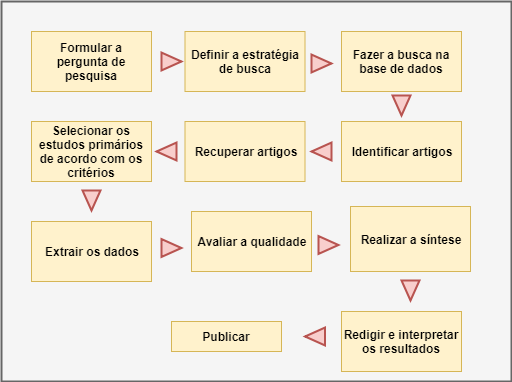
\includegraphics[scale=0.6]{figuras/sistematica.png}
	\end{center}
	\label{fig:processoRevisao}
	\legend{Fonte: Adaptado de \cite{kitchenham}.}
\end{figure}



A revisão sistemática da literatura é o método de pesquisa adotado neste trabalho para coleta dos dados. No próximo capítulo, a metodologia deste trabalho é descrita.
